\section{Ejercicio 7}
\subsection{Enunciado}

\subsection{Soluci\'on}

%SI QUIEREN AGREGAR IMAGENES COPIEN EL SIGUIENTE CODIGO
%\begin {center}
%\includegraphics[width=12cm]{./graphEj1.jpg}
% grafico.eps: 0x0 pixel, 300dpi, 0.00x0.00 cm, bb=50 50 410 302
%\end {center}

\begin {center}
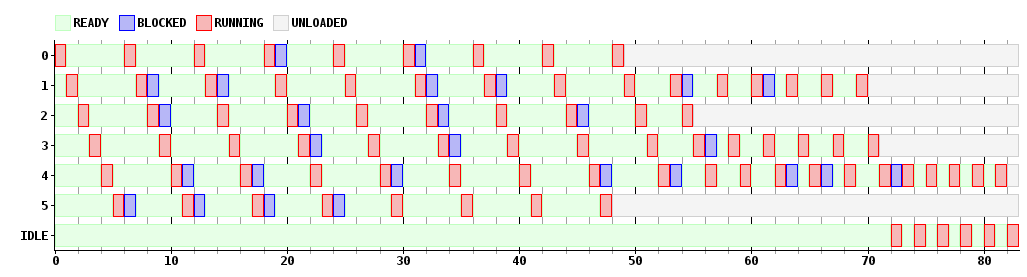
\includegraphics[width=12cm]{../simusched/outputs/ej7/rr-ej7-0-1.png}
grafico.eps: 0x0 pixel, 300dpi, 0.00x0.00 cm, bb=50 50 410 302
\end {center}

\begin {center}
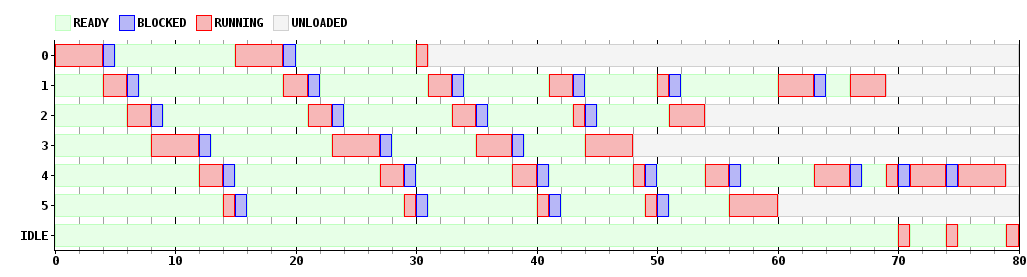
\includegraphics[width=12cm]{../simusched/outputs/ej7/rr-ej7-0-5.png}
grafico.eps: 0x0 pixel, 300dpi, 0.00x0.00 cm, bb=50 50 410 302
\end {center}

\begin {center}
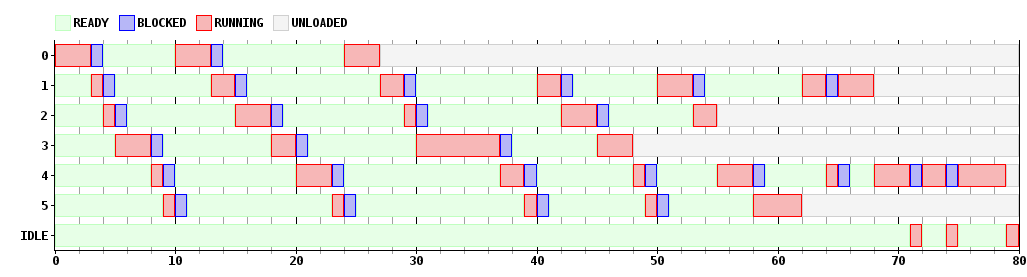
\includegraphics[width=12cm]{../simusched/outputs/ej7/rr-ej7-0-20.png}
grafico.eps: 0x0 pixel, 300dpi, 0.00x0.00 cm, bb=50 50 410 302
\end {center}


Laala
\begin {center}
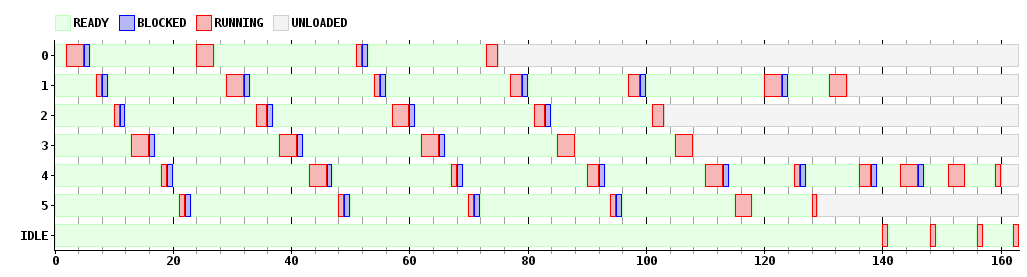
\includegraphics[width=12cm]{../simusched/outputs/ej7/rr-ej7-2-3.png}
\end {center}

\begin {center}
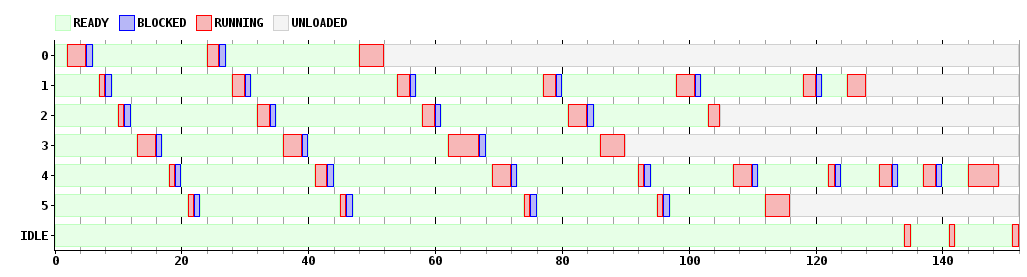
\includegraphics[width=12cm]{../simusched/outputs/ej7/rr-ej7-2-5.png}
grafico.eps: 0x0 pixel, 300dpi, 0.00x0.00 cm, bb=50 50 410 302
\end {center}

\begin {center}
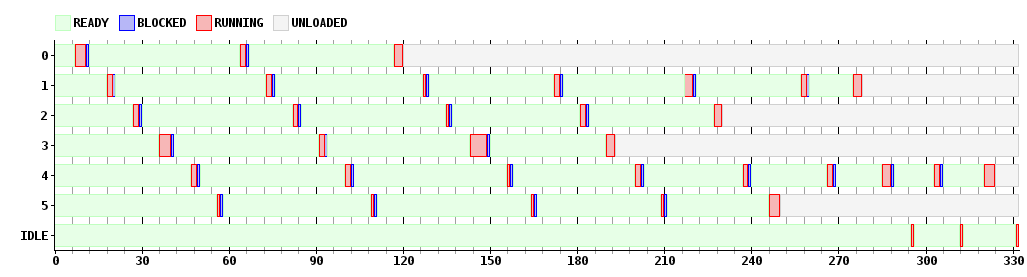
\includegraphics[width=12cm]{../simusched/outputs/ej7/rr-ej7-7-15.png}
grafico.eps: 0x0 pixel, 300dpi, 0.00x0.00 cm, bb=50 50 410 302
\end {center}
